\documentclass{beamer}
\DeclareFontShape{OT1}{cmss}{b}{n}{<->ssub * cmss/bx/n}{} 
\usetheme{CambridgeUS}
\usecolortheme{rose}
\usepackage{amsmath}
\usepackage{amsfonts}
\usepackage{mathbbol}
\usepackage{xcolor} % before tikz or tkz-euclide if necessary
\usepackage{tkz-euclide} % no need to load TikZ
\usepackage{multirow}
\usepackage{lmodern}
\usepackage{bm}
\usepackage{subcaption}
%\usepackage{subfigure}

\usepackage[
backend=biber,
style=authoryear-icomp,
sortlocale=de_DE,
natbib=true,
url=false, 
doi=true,
eprint=false
]{biblatex}
\addbibresource{../Bibliography/main_ML.bib}



\titlegraphic{
\includegraphics[width=2cm]{../Figures/UAMS_RGB.png}
}


\title{Connectomics: Null Hypotheses}
\author{Horacio G\'omez-Acevedo}

\begin{document}

	\begin{frame}[plain]
		\maketitle
	\end{frame}
\section{Introduction to Hypothesis Testing}	
\begin{frame}{Hypothesis Testing}
There are key components to take full advantage of th

\begin{itemize}
	\item Likelihood
	\item Statistical Hypothesis
	\item Hypothesis Test
	\item Likelihood Ratio
	\item Asymptotic Properties of the Normal Distribution
	\item $p$-values
\end{itemize}
\end{frame}
\begin{frame}{Likelihood}
	If we have $X_1,\ldots, X_n$ independent and identically distributed (iid) random variables with a common probability (mass/density) function $f(x;\theta)$ where the parameter $\theta$ is unknown ($\theta \in \Omega$). The likelihood of a sample $\vec{x}=(x_1,\ldots,x_n)$ is 
	\begin{equation*}
		L(\theta,\vec{x})= \prod_{i=1}^n f(x_i,\theta)
	\end{equation*}
Example: If we have $X_i \sim N(\theta,\sigma^2)$ with $\sigma^2>0$ known but $\theta$ unknown. Then
\begin{equation*}
L(\theta,\vec{x})= \left(\frac{1}{2\pi \sigma^2}\right)^{n/2}
\exp\left(- \frac{1}{2\sigma^2}\sum_{i=1}^n (x_i-\overline{x})^2\right)\exp\left(- \frac{1}{2\sigma^2}n(\overline{x}-\theta)^2\right)
\end{equation*}
\end{frame}

\begin{frame}{Statistical Hypothesis}
	A Statistical Hypothesis is a conjecture about the probability distribution of a population. 
	
Example: We suppose that in an experiment we have a random sample from $N(\theta,10)$. 
\begin{equation*}
	\begin{split}
		H_0 &\colon \text{ The population is } N(5,10) \text{-distributed}\\
		H_1 &\colon \text{ The population is } N(1,10) \text{-distributed}
	\end{split}
\end{equation*}
\end{frame}

\begin{frame}{Hypothesis Test}
	A Hypothesis Test is a tuple $(X_1,\ldots, X_n; H_0,H_1,G)$, where
	\begin{enumerate}
		\item $(x_1,\ldots, x_n)$ is a sample of $(X_1,\ldots, X_n)$ random variables iid.
		\item $H_0$ and $H_1$ are hypothesis concerning the probability distribution of the population.
		\item $G\subset \mathbb{R}^n$ is Borel set (countable unions of open sets). 
	\end{enumerate}
The \textbf{level of significance} is defined as 
\begin{equation*}
	\alpha = P^{H_0}_{X_1,\ldots, X_n}(G)
\end{equation*}
We will consider hypothesis such as
\begin{equation*}
	H_0\colon \theta=\theta_0 (\text{ or }\theta \in \Theta_0) \qquad H_1 \colon \theta\ne \theta_0 (\text{ or }\theta \in \Theta=\Theta_1\cup \Theta_0)
\end{equation*}

\end{frame}

\begin{frame}{Maximum Likelihood Test}
	The \textbf{likelihood ratio} function
	\begin{equation*}
		\Lambda(x_1,\ldots,x_n)= \frac{\sup_{\theta\in \Theta_0}L_\theta(x_1,\ldots,x_n)}{\sup_{\theta\in \Theta} L_\theta(x_1,\ldots, x_n)}
	\end{equation*}
Let $\widehat{\theta}$ be the maximum likelihood estimate of $\theta$. 

If $\theta_0$ is the true value of $\theta$, then $L(\theta_0)$ is the maximum value of $L(\theta)$. Since $\Lambda \le 1$, then if $H_0$ is true $\Lambda $ should be close to 1, whereas if $H_1$ is true then $\Lambda$ should be smaller. 

We have the decision rule
\begin{equation*}
	\text{Reject } H_0 \text{ in favor of } H_1 \text{ if }\Lambda \le c,
\end{equation*}
where $\alpha= P^{\theta_0}(\Lambda \le c)$.
\end{frame}

\begin{frame}{Asymptotic Properties}
	Under some (regularity)conditions we have the following result:
	
	If the null hypothesis $H_0\colon \theta= \theta_0$.
	\begin{equation*}
		-2 \log \Lambda(X_1,\ldots, X_n) \to \chi^2(1)
	\end{equation*}
	\begin{figure}[h]
		\centering
		%	\begin{subfigure}{0.4\textwidth}
			%		\centering
			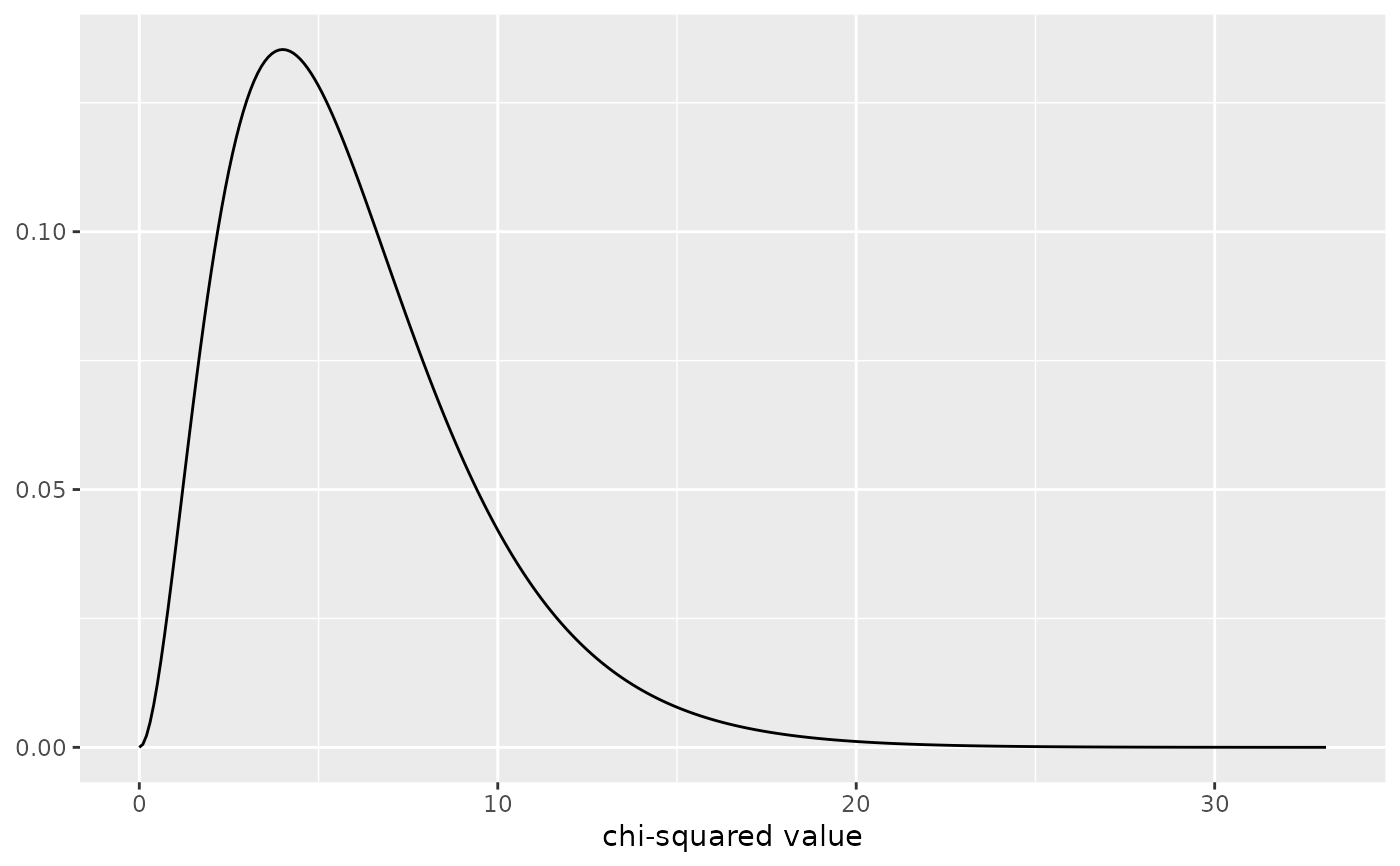
\includegraphics[scale=0.45]{../Figures/fig_chi_square1.png}
			%	\end{subfigure}
	\end{figure}
	
	
\end{frame}

\begin{frame}{Asymptotics for the Normal distribution}
	When $\mu$ and $\sigma$ are unknown and testing the hypothesis
	\begin{equation*}
		H_0 \colon \mu=\mu_0 \quad H_1 \colon \mu \ne \mu_0
	\end{equation*}
The likelihood ratio is given by
\begin{equation*}
	\Lambda(x_1,\ldots, x_n)= \left\{ 1+ \frac{1}{n-1}\left( \frac{\overline{x}-\mu_0}{s/\sqrt{n}}\right)\right\}^{-n/2}
\end{equation*}
where $s^2= \frac{1}{n-1}\sum_{i}(x_i-\overline{x})^2$. The critical regions are of the form
\begin{equation*}
	G= \{ (x_1,\ldots, x_n)\in \mathbb{R}^n: \left|\frac{\overline{x}-\mu_0}{s/\sqrt{n}} \right|\ge c\}
\end{equation*}
\end{frame}
\begin{frame}{$p$-values}
	The test statistic $\frac{\overline{x}-\mu_0}{s/\sqrt{n}}$ is critical to reject $H_0$ or not. The decision procedure is as follows
	\begin{equation*}
		\begin{split}
		\text{if }&\left| \frac{\overline{x}-\mu_0}{s/\sqrt{n}} \right| \ge c \text{ then we assume }H_1\\
			\text{if }&\left| \frac{\overline{x}-\mu_0}{s/\sqrt{n}} \right| <c \text{ then we assume }H_0
		\end{split}
	\end{equation*}
Furthermore, we have the following equivalence
\begin{equation*}
	P\left(	\left| \frac{\overline{x}-\mu_0}{s/\sqrt{n}} \right| \ge u \right)\le \alpha \iff u \ge c
\end{equation*}
The $p$-value associated with the outcome $u$ of the test statistic $\frac{\overline{x}-\mu_0}{S/\sqrt{n}}$ 
\begin{equation*}
	P\left(	\left| \frac{\overline{x}-\mu_0}{s/\sqrt{n}} \right| \ge |u| \right)
\end{equation*}
\end{frame}

\begin{frame}{$p$-values (cont)}
	Thus if an outcome $u$ of $\frac{\overline{x}-\mu_0}{S/\sqrt{n}}$  satisfies 
	\begin{equation*}
		P\left(	\left| \frac{\overline{x}-\mu_0}{s/\sqrt{n}} \right| \ge |u| \right) \le \alpha \text{ we accept }H_1
	\end{equation*}
	
\end{frame}

	\begin{frame}{Today's paper}
		\begin{figure}[h]
			\centering
			%	\begin{subfigure}{0.4\textwidth}
				%		\centering
				
\includegraphics[scale=0.45]{../Figures/fig_brunton_paper.png}
				%	\end{subfigure}
		\end{figure}
	\end{frame}
	
	
	\begin{frame}{Background}
		What are eigenvalues and eigenvectors?
		
		Let $A$ be a $n\times n$ matrix  (real), a number $\lambda \in \mathbb{C}$ is an \textbf{eigenvalue} if there is a nonzero vector $x \in \mathbb{C}^n$ for which $Ax= \lambda x$. We call such a vector an \textbf{eigenvector} of $A$ associated with $\lambda$. 
		
		The collection of all eigenvalues of $A$ is called the \textbf{spectrum} of $A$.
		
		The fundamental theorem for linear systems: If $A$ is a $n\times n$ matrix. For any $x_0 \in \mathbb{R}^n$, the initial value problem 
		\begin{equation*}
			\dot{x}=A x \qquad x(0)=x_0
		\end{equation*}
		has a unique solution
		\begin{equation*}
			x(t)= \exp(A^t)x_0
		\end{equation*}
		
	\end{frame}
	
	
	\begin{frame}{Eigenvalues in Dynamical Systems}
		\begin{figure}[h]
			\centering
			%	\begin{subfigure}{0.4\textwidth}
				%		\centering
				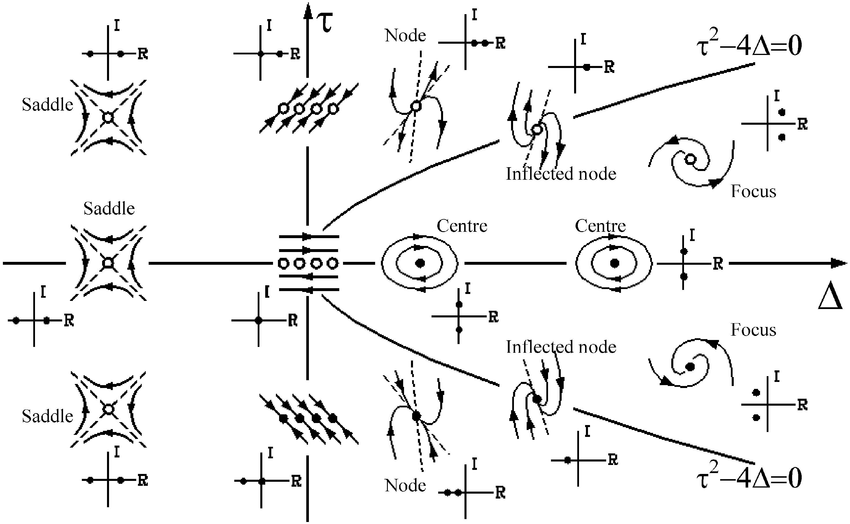
\includegraphics[scale=0.3]{../Figures/fig_phase_portrait.png}
				%	\end{subfigure}
		\end{figure}
		\url{https://www.researchgate.net/profile/Marco-Altosole/publication/245387409/figure/fig1/AS:392836487892996@1470670925920/Types-of-phase-portrait.png}		
	\end{frame}
	
	\begin{frame}{Singular Value Decomposition}
		If $A \in M_{m,n}$ has rank $k$, then it may be written in the form 
		\begin{equation*}
			A=V \Sigma W^*
		\end{equation*}
		where $V\in M_m$ and $W\in M_n$ are unitary ($W^* W=I_n$). The matrix $\Sigma=diag\{\sigma_1,\ldots, \sigma_q\}$ are the non-negative square roots of the eigenvalues of $AA^*$. The columns of $V$ are eigenvectors of $AA^*$, and the columns of $W$ are eigenvectors of $A^* A$. If $m\le n$ and if $AA^*$ has distinct eigenvalues, then $V$ is determined up to a right diagonal factor $D=diag( \exp(i\theta_1), \ldots, \exp(i \theta_n)$ where $\theta_j \in \mathbb{R}$. 
	\end{frame}
	
	\begin{frame}{Main Premise}
		The DMD algorithm seeks a best-fit linear matrix $A$ that approximately advances the state of a system $x\in \mathbb{R}^n$ forward in time according to the linear system
		\begin{equation*}
			x_{k+1}= A x_k
		\end{equation*}
		where $x_k= x(k\Delta t)$ and $\Delta t$ denotes a fixed time step that is small enough to resolve the highest frequencies in the dynamics.
	\end{frame}
	
	\begin{frame}{DMD setup }
		\begin{figure}[h]
			\centering
			%	\begin{subfigure}{0.4\textwidth}
				%		\centering
				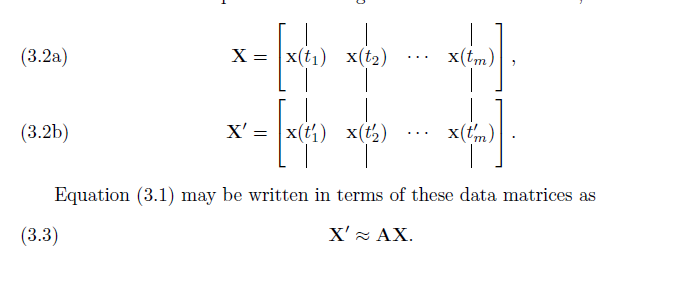
\includegraphics[scale=0.6]{../Figures/fig_dmd_fig1.png}
				%	\end{subfigure}
		\end{figure}
	\end{frame}
	
	\begin{frame}{DMD trick}
		\begin{figure}[h]
			\centering
			%	\begin{subfigure}{0.4\textwidth}
				%		\centering
				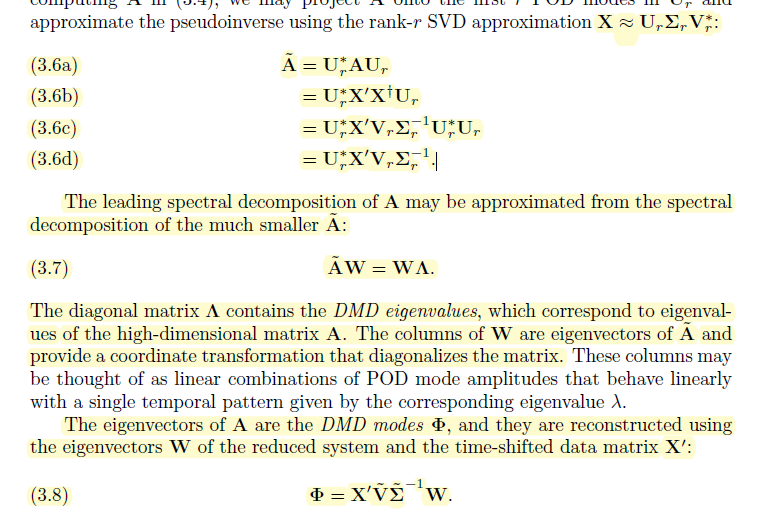
\includegraphics[scale=0.6]{../Figures/fig_dmd_fig2.png}
				%	\end{subfigure}
		\end{figure}	
	\end{frame}
	
	\begin{frame}{DMD expansion}
		\begin{figure}[h]
			\centering
			%	\begin{subfigure}{0.4\textwidth}
				%		\centering
				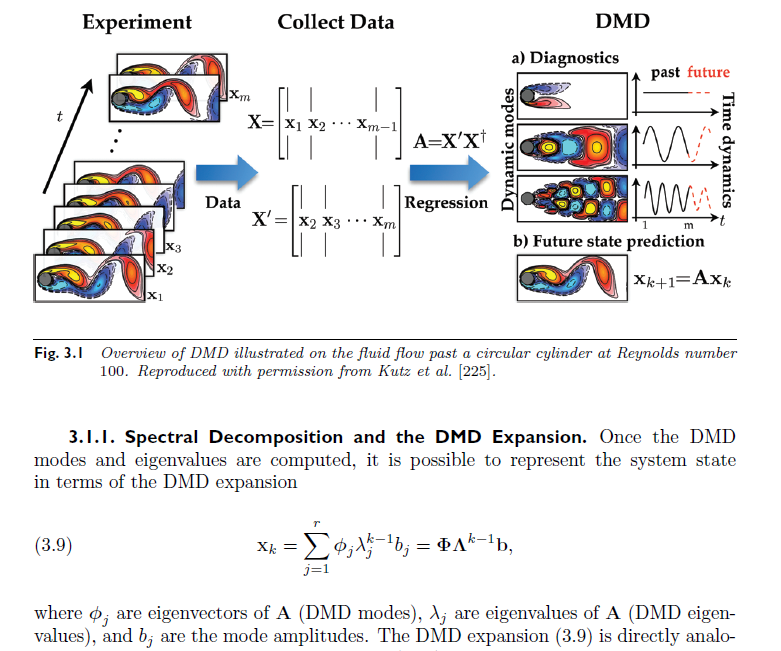
\includegraphics[scale=0.5]{../Figures/fig_dmd_fig3.png}
				%	\end{subfigure}
		\end{figure}	
	\end{frame}
	
	\begin{frame}{DMD expansion (cont)}
		\begin{figure}[h]
			\centering
			%	\begin{subfigure}{0.4\textwidth}
				%		\centering
				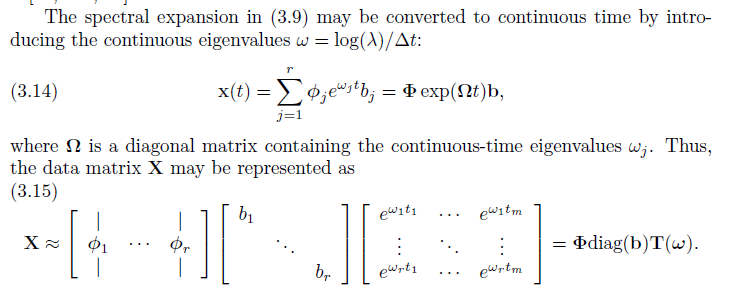
\includegraphics[scale=0.5]{../Figures/fig_dmd_fig4.png}
				%	\end{subfigure}
		\end{figure}	
	\end{frame}
	
	
	
	\begin{frame}{Colophon}
		\begin{figure}[h]
			\centering
			%	\begin{subfigure}{0.4\textwidth}
				%		\centering
				
\includegraphics[scale=0.35]{../Figures/siam_new.jpg}
				%	\end{subfigure}
		\end{figure}	
	\end{frame}	
	
	
	
	%\begin{frame}{Fourier Transform}
	%	\begin{figure}[h]
		%	\centering
		%	%	\begin{subfigure}{0.4\textwidth}
			%		%		\centering
			%		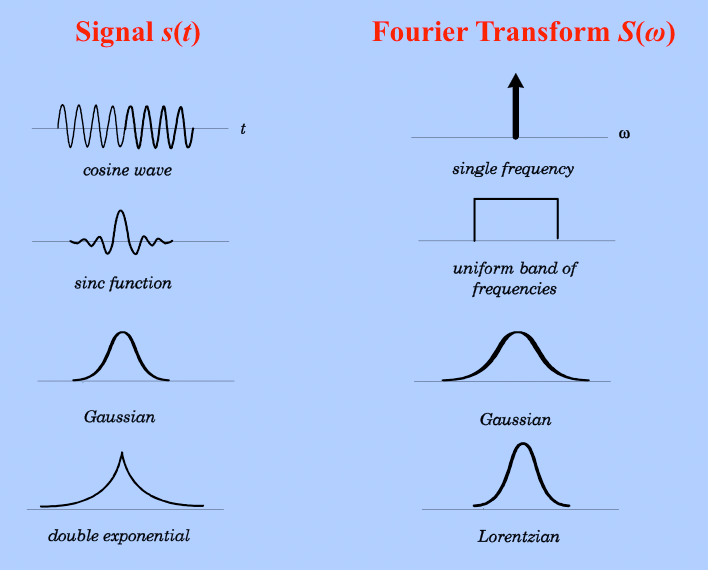
\includegraphics[scale=0.65]{../Figures/fig_fourier_transform.}
			%		%	\end{subfigure}
		%\end{figure}
		%\end{frame}
		
		
		%\begin{frame}{References}
		%	Materials and some of the pictures are from \citep{calin}.
		%	\printbibliography 	
		
		%	I have used some of the graphs by hacking TiKz code from StakExchange, Inkscape for more aesthetic plots and other old tricks of \TeX
		
		%\end{frame}
		
		
	\end{document}
